\paragraph{\trDoubleCover{}中的\trVanishingCycle{}与\trMatchingCycle{}。}\label{sub:vanishing-matching-double-cover}
取 $\pi$ 的一条\trVanishingPath{}$\gamma\colon[0;1]\to S$，起点为 $\gamma(0)=*$，并且整条落在较小的\trDisk{}$\scr{W}\subset S$ 之内。由于 $\Psi\colon\widetilde{\scr{E}}\to\scr{W}$ 与 $\pi$ 有相同的\trCriticalValue，我们也可以把 $\gamma$ 想成那一\trLefschetzFibration{}的\trVanishingPath，因而存在一个相伴的\trVanishingCycle{}$\widetilde{V}_\gamma$，它是 $\widetilde{E}=\widetilde{\scr{E}}_*$ 中的一个\trLagrange\trSphere。另一方面，我们在\cref{sub:double-branched-cover}中已经看到，$\gamma$ 的\trPreimage{}经适当的\trParametrization{}便成为 $\tilde{\gamma}\colon[-1;1]\to\widetilde{S}$，它是 $\tilde{\pi}$ 的一条\trMatchingPath，相伴的\trMatchingCycle{}为 $\widetilde{\Delta}_\gamma$。
\begin{lemma}\label{thm:matching-vanishing-isotopy}
作为 $\widetilde{E}$ 中带\trFrame{}的\trLagrange\trSphere，$\widetilde{\Delta}_\gamma$ \trIsotopy{}于 $\widetilde{V}_\gamma$。
\end{lemma}
\begin{proof}
这一论断的大部分都可以从\trBifibration{}的一般理论——更具体地说，\cref{thm:vanishing-as-matching-cycle}——导出。也就是说，考察 $\mathrm{Critv}(\varpi)\subset\widetilde{\scr{S}}$ 的结构（见 \eqref{eq:family-crit-sets}），便可看出与 $\gamma$ 相伴的那条\trMatchingPath\trIsotopy{}于 $\tilde{\gamma}$。这一论证的唯一问题在于，\cref{thm:vanishing-as-matching-cycle}并未刻画所出现的那个\trIsotopy{}$I$。当然，在当前情形下，由于\trMatchingCycle{}可以按朴素方式来构造，这个\trIsotopy{}多少是多余的；不过，检查一下所有这些要素是否恰当地凑在了一起，也许仍值得一做。按惯常的做法，我们先在唯一的\trCriticalPoint{}$x\in E_z$（$z=\gamma(1)$）附近作一个局部\trDeformation，使\trKaehler{}形式 $\phi_E$ 在局部\trHolomorphic{}\trMorse{}坐标中成为标准的。我们还可以假定：当 $t$ 接近 $1$ 时，$\gamma(t)=z+(1-t)$。这两处改动都是允许的，因为它们不影响所论的两个带\trFrame{}的\trLagrange\trSphere{}的\trIsotopy{}类。取短的\trVanishingPath{}$\gamma|[s;1]$（$s$ 充分接近 $1$）以及它在 $\scr{S}_{\gamma(s)}\to S$ 之下的\trPreimage——后者是 $\varpi_{\gamma(s)}$ 的一条\trMatchingPath。按假定，这个\trPreimage{}恰恰就是连接 $z-\gamma(s)$ 的两个平方根的那条直线。
取如 \eqref{eq:local-morse-equation} 中的局部坐标 $(y,x)$，于是 $\phi_{\widetilde{\scr{E}}}=d\kappa+\phi_E+\Psi^*\phi_{\scr{W}}$，其中如今第二个被加项是 $x$-坐标中的标准形式。这并不是 $\CC^{n+2}$ 上的标准形式，但由 $y\in i\RR$、$x\in\RR^{n+1}$ 所定义的子空间仍然是 $\phi_{\widetilde{\scr{E}}}$-\trLagrange{}的。从我们对\trLefschetzThimble{}的刻画容易看出，这个子空间的适当一部分必然是 $\gamma|[s;1]$ 的\trLefschetzThimble；于是，\trVanishingCycle{}为
\begin{equation}\label{eq:vanishing-cycle-short-path}
\widetilde{V}_{\gamma|[s;1]}=\{y\in i\RR,\ x\in\RR^{n+1},\ |y|^2+|x|^2=\gamma(s)-z\},
\end{equation}
带有显然的\trFrame。到目前为止，我们一直把 $\gamma|[s;1]$ 当作 $\Psi$ 的\trVanishingPath{}来看待。如果现在暂时回到把它看作 $\pi$ 的\trVanishingPath{}的观点，那么相应的\trLefschetzThimble{}当然是 $\{x\in\RR^{n+1},\ |x|^2\le\gamma(s)-z\}$；于是，这个\trLefschetzThimble{}在 $\beta_{\widetilde{\scr{E}}}|\widetilde{\scr{E}}_{\gamma(s)}$ 之下的\trPreimage——按定义即 $\widetilde{\Delta}_{\gamma|[s;1]}$——与 \eqref{eq:vanishing-cycle-short-path} 相重合。如同\cref{thm:vanishing-as-matching-cycle}中那样，现在再借适当的\trParallelTransport{}映射把这个事实传送回整条路径 $\gamma$。
\end{proof}
为了将来引用，我们再来考察两个别的几何情形，它们仍涉及上面所定义的那些\trLagrange\trSubmanifold{}类。设给定了 $\pi$ 的三条\trVanishingPath{}$\gamma_k$、$\gamma_{k+1}$、$\delta_k$，如\cref{fig:hurwitz-move}中那样（当然，在这一点上我们并不需要整个\trDistinguishedBasis，不过为方便起见仍沿用那一记号）。把 $\widetilde{E}$ 中与之相伴的 (B) 型\trLagrange\trSubmanifold{}记作 $\widetilde{\Delta}_k$、$\widetilde{\Delta}_{k+1}$、$\widetilde{\Pi}_k$。
\begin{lemma}\label{thm:type-b-dehn-twist-isotopy}
作为 $\widetilde{E}$ 中带\trFrame{}的\trLagrange\trSphere，$\widetilde{\Pi}_k$ \trIsotopy{}于 $\tau_{\widetilde{\Delta}_k}(\widetilde{\Delta}_{k+1})$。
\end{lemma}
\begin{proof}
不失一般性，可以假定这些路径都含于 $\scr{W}$ 之内。于是，按\cref{thm:matching-vanishing-isotopy}，$\widetilde{\Delta}_k$ 就是把 $\gamma_k$ 当作 $\Psi$ 的\trVanishingPath{}来看待时的那个\trVanishingCycle。因此，与之相伴的\trDehnTwist{}便是 $\Psi$ 沿一条把该路径加倍的\trLoop{}$\lambda$ 的\trMonodromy，这意味着
\begin{equation*}
\tau_{\widetilde{\Delta}_k}(\widetilde{\Delta}_{k+1})\simeq h_\lambda(\widetilde{\Delta}_{k+1}).
\end{equation*}
按定义，$\delta_k$ 是取 $\gamma_{k+1}$ 而把它的起点沿 $\lambda$ 移动所得的结果。这意味着存在一族 $\pi$ 的\trSmooth{}\trVanishingPath{}$\gamma^s$，满足 $\gamma^s(0)=\lambda(s)$、$\gamma^s(1)=\gamma_{k+1}(1)$，它始于 $\gamma^0=\gamma_{k+1}$ 而终于 $\gamma^1=\delta_k$。这些路径给出一个由带\trFrame{}的\trLagrange\trSphere{}组成的\trSmooth{}族 $\widetilde{\Delta}^s\subset\widetilde{\scr{E}}_{\lambda(s)}$，在 $\widetilde{\Delta}^0=\widetilde{\Delta}_{k+1}$ 与 $\widetilde{\Delta}^1=\widetilde{\Pi}_k$ 之间\trInterpolation。考察这些\trSphere{}沿 $\lambda|[s;1]$ 在\trParallelTransport{}之下的像，便得到 $h_\lambda(\widetilde{\Delta}_{k+1})$ 与 $\widetilde{\Pi}_k$ 之间的一个\trIsotopy。
\end{proof}
最后，设 $\mu$ 是 $\pi$ 的一条\trMatchingPath，并设 $\Sigma_\mu\subset E$ 是它的\trMatchingCycle。按假定，负\trLiouville{}流会把每个\trLagrange\trSubmanifold{}送入 $E^{\mathrm{shrink}}$ 之内；而既然 $\Sigma_\mu$ 只是在相差\trIsotopy{}的意义下定义的，我们不妨干脆假定它含于 $E^{\mathrm{shrink}}$ 之内，于是它的\trPreimage{}$\widetilde{\Sigma}_\mu=\widetilde{\Sigma}_{\mu,+}\cup\widetilde{\Sigma}_{\mu,-}$ 是一个 (U) 型\trLagrange\trSubmanifold，由 $\widetilde{E}$ 中两个不交的带\trFrame{}的\trLagrange\trSphere{}组成。取\trVanishingPath{}$\gamma_k$、$\gamma_{k+1}$，二者都始于 $*$ 而终于 $\mu$ 的两个端点，如\cref{fig:matching-triangle}中那样。关键的要求是：这三条路径所描出的三角形，其内部不得含有 $\pi$ 的任何\trCriticalValue，这使得\trComposition{}路径 $\gamma'_{k+1}=\mu\#\gamma_k$（按与\cref{sub:concatenation-paths}中相同的方式构成）成为一条\trIsotopy{}于 $\gamma_{k+1}$ 的\trVanishingPath。设 $\widetilde{\Delta}_k$、$\widetilde{\Delta}_{k+1}$ 是与 $\gamma_k$、$\gamma_{k+1}$ 相伴的 (B) 型\trSubmanifold。
\begin{lemma}\label{thm:type-b-double-twist-isotopy}
作为带\trFrame{}的\trLagrange\trSphere，$\widetilde{\Delta}_{k+1}$ \trIsotopy{}于 $\tau_{\widetilde{\Sigma}_{\mu,-}}\tau_{\widetilde{\Sigma}_{\mu,+}}(\widetilde{\Delta}_k)$。
\end{lemma}
\begin{figure}[htbp]
\centering
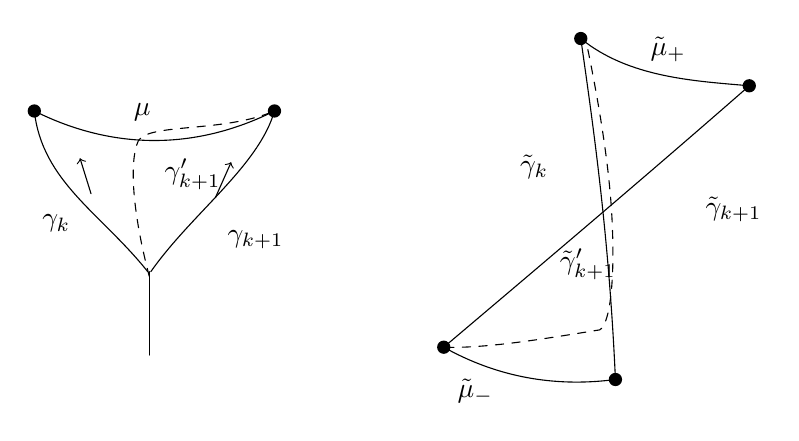
\begin{tikzpicture}[line cap=round,line join=round,scale=1.0]
\fill (0,3.0) circle (2.4pt);%
\fill (3.05,3.0) circle (2.4pt);%
\draw (0,3.0) .. controls (1.0,2.5) and (2.05,2.5) .. (3.05,3.0);%
\draw (1.46,0.96) -- (1.46,-0.1);%
\draw (1.44,0.96) .. controls (0.85,1.7) and (0.1,2.1) .. (0,3.0);%
\draw (1.48,0.96) .. controls (2.0,1.7) and (2.85,2.3) .. (3.05,3.0);%
\draw[->] (0.72,1.95) -- (0.58,2.4);%
\draw[->] (2.3,1.9) -- (2.5,2.35);%
\draw[dashed] (1.46,0.9) .. controls (1.25,1.7) and (1.2,2.35) .. (1.32,2.62) .. controls (1.45,2.85) and (2.4,2.72) .. (3.05,3.0);%
\node[anchor=south] at (1.37,2.75) {$\mu$};
\node[anchor=west] at (1.53,2.2) {$\gamma'_{k+1}$};
\node[anchor=east] at (0.58,1.57) {$\gamma_k$};
\node[anchor=west] at (2.33,1.36) {$\gamma_{k+1}$};
\begin{scope}[xshift=5.2cm]
\fill (1.74,3.92) circle (2.4pt);%
\fill (3.88,3.32) circle (2.4pt);%
\fill (0,0) circle (2.4pt);%
\fill (2.18,-0.41) circle (2.4pt);%
\draw (1.74,3.92) .. controls (2.35,3.42) and (3.2,3.38) .. (3.88,3.32);%
\draw (0,0) .. controls (0.75,-0.42) and (1.5,-0.5) .. (2.18,-0.41);%
\draw (1.74,3.92) .. controls (1.9,2.8) and (2.1,1.4) .. (2.18,-0.41);%
\draw (0,0) .. controls (1.3,1.1) and (2.6,2.2) .. (3.88,3.32);%
\draw[dashed] (1.83,3.78) .. controls (2.02,2.85) and (2.12,2.1) .. (2.14,1.55) .. controls (2.17,0.9) and (2.12,0.3) .. (1.98,0.22) .. controls (1.35,0.12) and (0.55,-0.02) .. (0,0);%
\node[anchor=south] at (2.85,3.5) {$\tilde{\mu}_+$};
\node[anchor=north] at (0.4,-0.28) {$\tilde{\mu}_-$};
\node[anchor=east] at (1.45,2.29) {$\tilde{\gamma}_k$};
\node[anchor=west] at (3.2,1.75) {$\tilde{\gamma}_{k+1}$};
\node[anchor=west] at (1.35,1.05) {$\tilde{\gamma}'_{k+1}$};
\end{scope}
\end{tikzpicture}
\caption{}\label{fig:matching-triangle}
\end{figure}
\begin{proof}
把 $\widetilde{\mu}=\widetilde{\mu}_+\cup\widetilde{\mu}_-$ 以及 $\tilde{\gamma}_k$、$\tilde{\gamma}_{k+1}$、$\tilde{\gamma}'_{k+1}$ 记作相应各路径在 $\widetilde{S}$ 中的\trPreimage。它们都是 $\tilde{\pi}$ 的\trMatchingPath，而且
\begin{equation*}
\tilde{\gamma}_{k+1}\simeq\tilde{\gamma}'_{k+1}=\widetilde{\mu}_-\#(\widetilde{\mu}_+\#\tilde{\gamma}_k).
\end{equation*}
把\cref{thm:matching-concatenation-twist}应用两次便给出所需的结果，只是可能存在\trFrame{}方面的问题；但这很容易解决：对我们原先的\trLefschetzFibration{}$E$ 上的\trSymplectic\trConnection{}作\trDeformation，使得 $\mu$ 的\trMatchingCycle{}按朴素意义来构造（取常值的\trIsotopy{}$I$）。对\trMatchingPath{}$\tilde{\gamma}_k$、$\tilde{\gamma}_{k+1}$ 而言，诸\trIsotopy{}也是常值的，而这与证明\cref{thm:matching-concatenation-twist}时所用的\trLagrange\trConnectedSum{}论证\trCompatible。
\end{proof}
\begin{remark}\label{thm:involution-equivariant-remarks}
上面三个引理中的每一个都容许顾及\trInvolution{}$\iota_{\widetilde{E}}$ 的改进版本：
\begin{itemize}
\item \cref{thm:matching-vanishing-isotopy}中的\trIsotopy{}自然是\trEquivariant{}的，因为在局部模型中等号成立，而用于化归到该模型情形的\trDeformation{}与 $\iota_{\widetilde{E}}$ \trCompatible。
\item 对于\cref{thm:type-b-dehn-twist-isotopy}，只需使用\trPicard--\trLefschetz{}公式的\trEquivariant{}版本。我们想指出一个有用的附加细节。该\trIsotopy{}与 $\tau_{\widetilde{\Delta}_k}|\widetilde{\Delta}_{k+1}$ 的\trComposition{}给出一个\trEquivariant{}\trDiffeomorphism
\begin{equation}\label{eq:equivariant-diffeomorphism-type-b}
\widetilde{\Delta}_{k+1}\longrightarrow\widetilde{\Pi}_k,
\end{equation}
于是比较两个\trSphere{}内部\trFixedPoint{}集的\trCoorientation{}便是有意义的。这样的\trCoorientation{}自然对应于 $\widetilde{S}$ 中路径 $\tilde{\delta}_k$、$\tilde{\gamma}_{k+1}$ 的\trOrientation。论断是：两个\trCoorientation{}与 \eqref{eq:equivariant-diffeomorphism-type-b} \trCompatible，当且仅当\trIntersectionNumber{}$\tilde{\delta}_k\cdot\tilde{\gamma}_{k+1}$ 在唯一的公共点（$y=0$）处等于 $-1$。看出这一点的办法是取\cref{thm:type-b-dehn-twist-isotopy}证明中的那个\trLoop{}$\lambda$，并把 $\widetilde{E}$ 上相伴的\trMonodromy{}与 $\widetilde{S}$ 上的\trBraid{}单值加以比较。一般地，辫单值是一个保持 $\mathrm{Critv}(\tilde{\pi})$ 的 $\widetilde{S}$ 的\trDiffeomorphism，而在当前情形下它不过是沿 $\tilde{\gamma}_k$ 的一个\trHalfTwist。如果选取 $\tilde{\gamma}_{k+1}$ 的一个\trOrientation，并为其像 $\tilde{\delta}_k=t_{\tilde{\gamma}_k}(\tilde{\gamma}_{k+1})$ 配备诱导的\trOrientation，那么局部\trIntersectionNumber{}的确等于 $-1$，见\cref{fig:half-twist-intersection}。
\begin{figure}[htbp]
\centering
\begin{tikzpicture}[line cap=round,line join=round,scale=1.0]
\fill (0,0) circle (2.4pt);%
\fill (1.3,-1.28) circle (2.4pt);%
\fill (3.2,2.9) circle (2.4pt);%
\fill (4.4,1.6) circle (2.4pt);%
\draw (0,0) -- (4.4,1.6);%
\draw (1.3,-1.28) -- (3.2,2.9);%
\draw[->] (2.25,0.81) -- (2.48,1.31);%
\draw[->] (2.42,0.88) -- (2.99,1.09);%
\draw (0,0) .. controls (0.35,-0.8) and (0.6,-1.6) .. (1.15,-1.82)
      .. controls (1.7,-2.02) and (2.28,-1.6) .. (2.22,-0.8)
      .. controls (2.17,-0.15) and (2.2,0.4) .. (2.24,0.79)
      .. controls (2.28,1.35) and (2.35,2.05) .. (2.62,2.78)
      .. controls (2.9,3.5) and (3.55,3.62) .. (3.9,3.3)
      .. controls (4.25,2.98) and (4.36,2.3) .. (4.4,1.6);%
\node[anchor=south] at (1.0,0.62) {$\tilde{\gamma}_{k+1}$};
\node[anchor=east] at (1.7,-0.32) {$\tilde{\gamma}_k$};
\node[anchor=west] at (4.2,2.6) {$\tilde{\delta}_k=t_{\tilde{\gamma}_k}(\tilde{\gamma}_{k+1})$};
\end{tikzpicture}
\caption{}\label{fig:half-twist-intersection}
\end{figure}
\item 我们的\cref{thm:type-b-double-twist-isotopy}证明对这一目的而言并不理想，因为一次只作一个\trDehnTwist，破坏了对称性。不过，只需对论证作一个适当的改动即可弥补：先给出诸\trLagrange{}球（在 $E$ 中相对 $M$ 取）的\trIsotopy{}$\Delta_{k+1}\simeq\tau_{\Sigma_\mu}(\Delta_k)$，再把它\trLift{}到\trDoubleBranchedCover{}上去。
\end{itemize}
\end{remark}
